\documentclass[10pt]{article}
\usepackage{titlesec}
\usepackage[paper=letterpaper,margin=2cm]{geometry}
\usepackage{amsmath}
\usepackage{amssymb}
\usepackage{amsfonts}
\usepackage{newtxtext, newtxmath}
\usepackage{enumitem}
\usepackage[colorlinks,allcolors=cyan]{hyperref}
\usepackage{graphicx, float}

\let\oldthefigure\thefigure% Capture figure numbering scheme
\renewcommand{\thefigure}{S\oldthefigure}% Prefix figure number with S
\let\oldsection\section
\renewcommand{\section}{\clearpage\oldsection}

\title{Understanding the Free Energy Landscape of Phase Separation in Lipid Bilayers using Molecular Dynamics}
\author{Ashlin J. Poruthoor, Alan Grossfield}

\begin{document}
\maketitle

\section{Simulation details$^\dagger$}

\begin{center}
    \begin{tabular}{|c c c c|}
    \hline
        & & & \\ 
        & {DPPC-DAPC-CHOL} & DPPC-DLiPC-CHOL & DPPC-POPC-CHOL  \\
        & & & \\ 
            \begin{tabular}{@{}c@{}}Bilayer composition\end{tabular} & 
            \begin{tabular}{@{}c@{}}600:360:240 \\ (0.5:0.3:0.2)\end{tabular} &
            \begin{tabular}{@{}c@{}}828:540:576 \\ (0.42:0.28:0.3)\end{tabular} &
            \begin{tabular}{@{}c@{}}480:480:240 \\ (0.4:0.4:0.2)\end{tabular} \\
        & & & \\ 
        $\text{Water}^{\parallel}$ & 9000 PW Beads & 14580 PW Beads & 9000 PW Beads  \\ 
        & & & \\ 
            \begin{tabular}{@{}c@{}}Temperatures for \\ std. MD \\ production runs \end{tabular} & 
            \begin{tabular}{@{}c@{}}298K, 323K, 333K, \\ 333K, 343K, 353K, \\ 373K, 423K, 450K \end{tabular} &
            \begin{tabular}{@{}c@{}}298K, 323K \\ 353K, 423K \\ 450K \end{tabular} &
            \begin{tabular}{@{}c@{}}298K, 323K, \\ 450K \end{tabular} \\
        & & & \\ 
            \begin{tabular}{@{}c@{}}Temperatures for \\ WE MD \\ production runs \end{tabular} & 
            \begin{tabular}{@{}c@{}}298K, 323K, 333K, \\ 333K, 343K, 353K, \\ 373K, 423K \end{tabular} &
            \begin{tabular}{@{}c@{}}298K, 323K \\ 353K, 423K \end{tabular} &
            \begin{tabular}{@{}c@{}}298K, 450K \\ \end{tabular} \\
        & & & \\ \hline
    \end{tabular}
\end{center}

\begin{center}
    \begin{tabular}{|c c|}
    \hline
        & \\ 
        Temperature &
            \begin{tabular}{@{}c@{}}Initial NPT equilibration @ 400 K, with Berendsen for 100 ns. \\
                 Production run at with v-rescale, $\tau$ = 1.0 ps\end{tabular} \\
        & \\ 
        Time step & 20 fs \\
        & \\ 
        vdW & Potential-shift-verlet. Cutoff = 1.1 nm. \\
        & \\ 
        \ \ \ Electrostatics \ \ \  & 
            \begin{tabular}{@{}c@{}} Reaction field. Cutoff = 1.1 nm\\
                Rel.dielectric constant = 2.5 (Since we are using polarizable water) \end{tabular} \\
        & \\ 
        Pressure & 
            \begin{tabular}{@{}c@{}} Parrinello-Rahman @ 1 bar. Semi isotropic.\\
                $\tau$ = 12 ps. Compressibility = 3 $\times 10^{-4}$ \end{tabular} \\
        & \\ 
    \hline
    \end{tabular}
\end{center}

$^\dagger$ The system parameters were obtained from the .mdp file for production stage which is given by CHARMM GUI\cite{Qi2015}
after building the system. These parameters agree with the MARTINI recommended parameters\cite{DeJong2016} for a CG lipid system that uses polarizable water\cite{Yesylevskyy2010}.
$^{\parallel}$ PW : Polarizable Water.

\section{Membrane restrain protocol}

Membrane undulation is a known behavior in large lipids bilayer system with large box vectors and membrane restrain protocols have been used to prevent them\cite{Ingolfsson2014,Lin2019,Su2020}.
There are two common protocols that have been used previously: (a) position restraining a certain bead of specific lipid or
(b) applying a flat bottom restraining on the membrane.
For detailed explanation of how this is implemented, refer to the GROMACS manual\cite{GromacsManual}.
Since the objective of the FLOPSS pipeline is to estimate free energy landscape of phase separating lipid bilayers,
we went for a less invasive restraining protocol.
We chose flat bottom restraints where the lipid bilayer can move in the xy slab of predefined z thickness.
Thus starting from the last 100 ns of NPT equilibration of lipid bilayer to the whole production run,
we introduced a flatbottom restraint to the bilayer.\\

There are two parameters to choose : (a) How thick should be the planar slab where bilayer is free to move, and
(b) What should be the force constant to be used for the flat bottom potential
In order to decide on the former, we found the mass density distribution of NC3, PO4 and GL1 beads along z direction using all four replicas.
We checked the mass density distribution at different steps of CHARMM-GUI suggested protocol.
The rationale was to check the bead to bead sitance of each lipid species and use this distance to set the radius od flatbottom well.
Based on the distributions at equilibration step, for the DPPC-DIPC-CHOL, we chose 2.3125 nm as the flat bottom well radius, with respect to PO4 bead of DPPC and DIPC.
For the DPPC-DAPC-CHOL, we chose 2.5625 nm as the flat bottom well radius, with respect to PO4 bead of DPPC and DAPC.
We chose PO4 bead since the head group choline (NC3) seemed more flexible (as instead of a sharp peaks at each leaflets it has a more broader peaks at each sides of the plots), therefore for the NC3 bead average value has more uncertainity to it.
Also, PO4 bead to bead distance for DPPC and D(A/I)PC was different but we went with the idea of one height for both, at the outer edge of the farther one.
Also we only applied the flatbottom restraints for the longer DPPC and D(A/I)PC lipids and not for cholesterol.
We also tested flat bottom restrain radius = 21 A, 22 A, 23 A, 24 A, 25 A, 26 A, 27 A for DIPC system and checked whether the criteria we chose prevented bilayer undulation just right while not making bilayer extra stiff.
By eyeballing through these systems, it seems our choice of criteria is just right.
We tried flat bottom restrain with force constant, k = 0.2, 2, 10, 20, 100, 200, 500, 1000, 2000, 3000 KJ mol-1nm-2 for DIPC system.
We ran 100 ns NPT runs and observed that the system seems to be undulating below 1000 mol-1 nm-2. 
Subsequent literature review of membrane restraining strategies among recent works, we found that in Su J. et al. (2020), where they used similar system, they have done a reference simulation and used as an alternative flat-bottomed potential restraint of 1000 KJ mol-1 nm-2, confining glycerol moieties to a xy slab of defined (4 nm) vertical thickness.
There is a close agreement in our choice of k and bead to bead distance that we observed for GL1 beads, with that of Su J. et al.
Thus we chose k = 1000 KJ mol-1 nm-2.


\section*{Radius cutoff calculations for $\epsilon$}

\begin{figure}[hbt!]
    \centering
    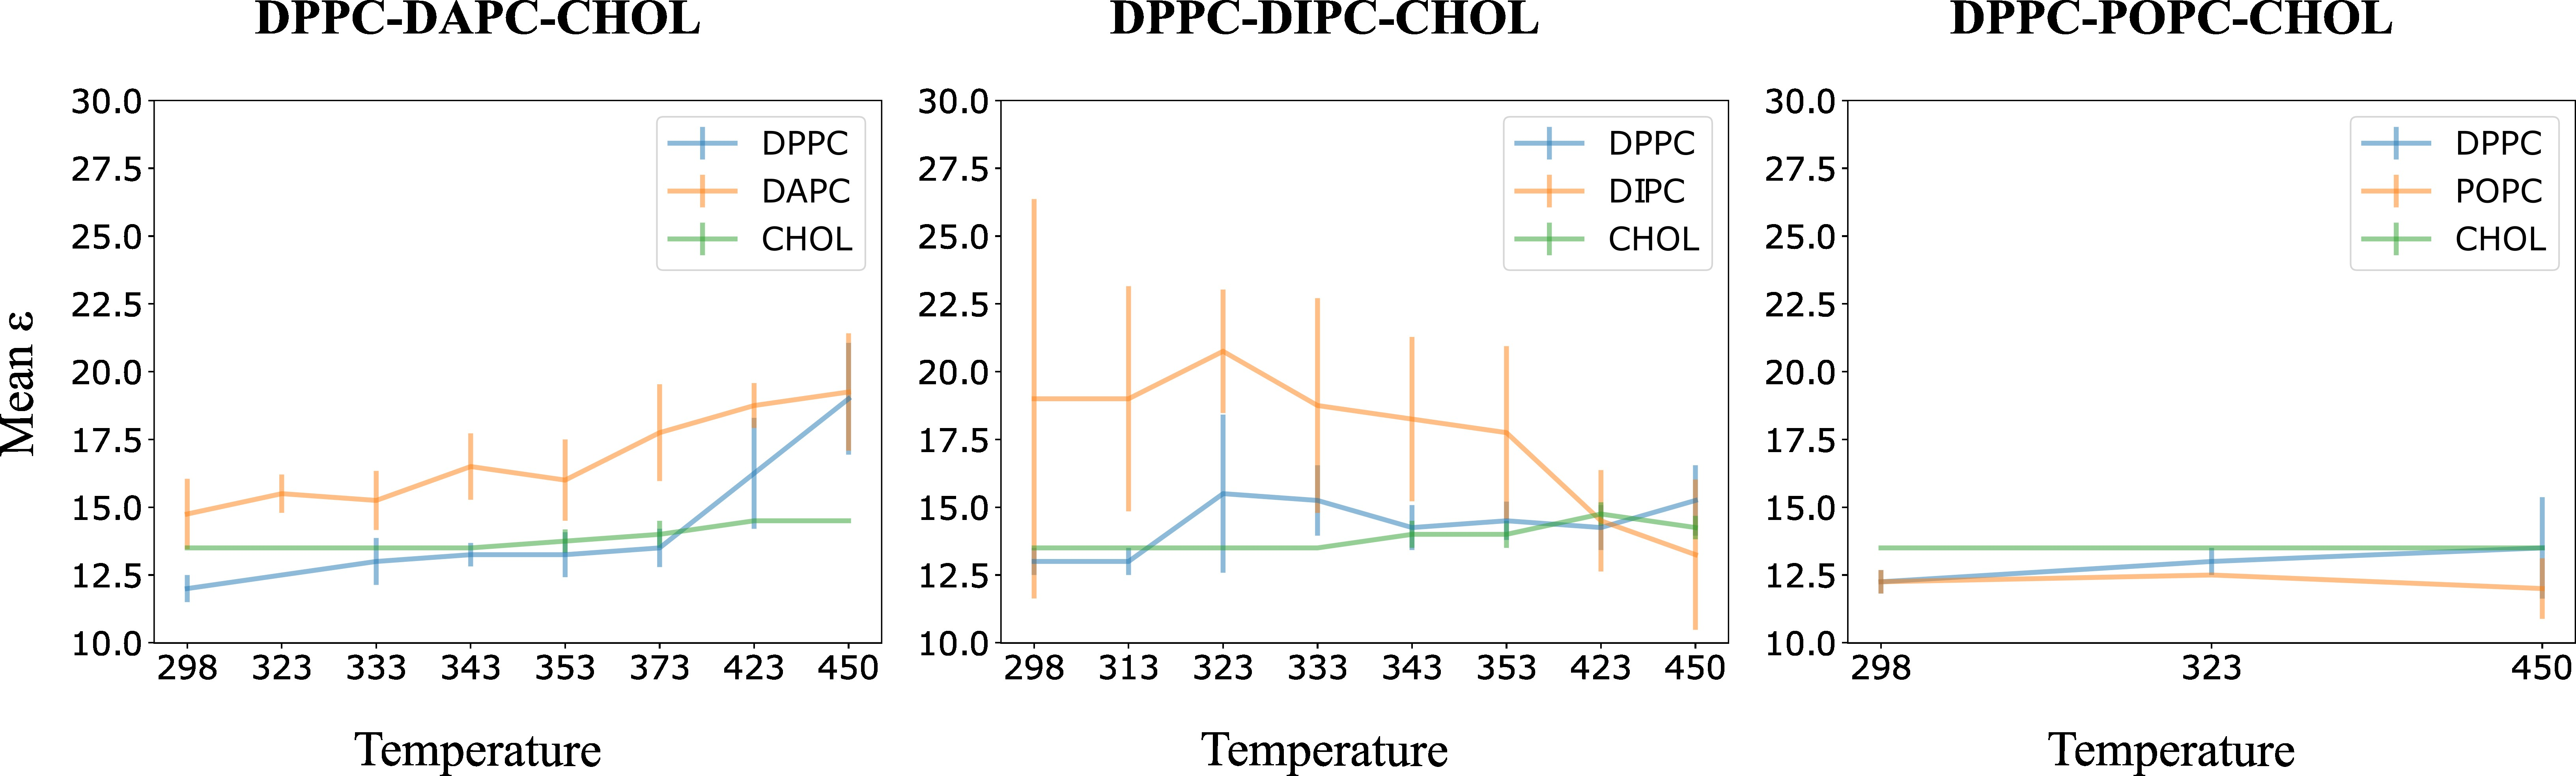
\includegraphics[width=6.5in]{Figures/Supplementary/epsilon/placeholder.jpg}
    \caption{Mean $\epsilon$ calculated using the \textit{xy\_rdf} tool in LOOS package at different temperature and for different lipid species in each system under study.}
    \label{figs1:view}
\end{figure}

\section*{Auxiliary variables}

To assess the quality of DBSCAN clustering, for each lipid species, $X_i$ in the system, we calculated the following, 

1. Number of $X$ clusters in the system under study.

2. Fraction of $X_i$ lipids in $X$ clusters

3. Fraction of $X_i$ lipids in $X$ core lipids.

4. Mean Silhouette Coefficient (MSC) of $X_i$ Clusters, as implemented in scikit-learn.

Silhouette Coefficient is a method used to evaluate the clustering done by any technique, especially if ground truth labels are unknown. 
Here, for a $X_i$ lipid in the cluster, mean intra-cluster distance (a) from other $X_i$ lipids in the cluster is found.  
Similarly, for a $X_i$ lipid in the cluster, the mean nearest-cluster distance (b) is also calculated.
While the former assesses the 'cohesion' of a given $X_i$ lipids with other $X_1$ lipids in a cluster, the latter assesses the 'separation' from the nearest cluster.
Thus, Silhouette Coefficient for a $X_i$ lipid, s, is defined as below,

\begin{equation}
\label{eq:SC}
\text{s} = \frac{b - a}{max(a,b)}
\end{equation}

The Mean Silhouette Coefficient of $X_i$ Clusters is given by the mean $s$ over all non-outlier $X_i$ lipids.
Here, we have omitted the MSC calculations for cases when there are no clusters or just one cluster detected by DBSCAN. 
MSC is bound between and -1 and 1.
A high positive value corresponds to well segregated dense clusters, while a low negative value implies that lipids are assigned to clusters incorrectly.  

All these AVs were tracked along with the primary collective varibale, FLC, driving the WE simulation.
Following are the system specific profiles of each AVs: 

\begin{figure}[H]
    \centering
    \includegraphics[width=6.5in]{Figures/Supplementary/AVs/ClusterCount/placeholder.jpg}
    \caption{Cluster count profile for each system as a function of temperatures. Each column represents each lipid system under study. The rows represent the total cluster count, saturated lipid cluster count, unsaturated cluster count and cholesterol cluster count within each system respectively}
    \label{figs2:view}
\end{figure}

\begin{figure}[H]
    \centering
    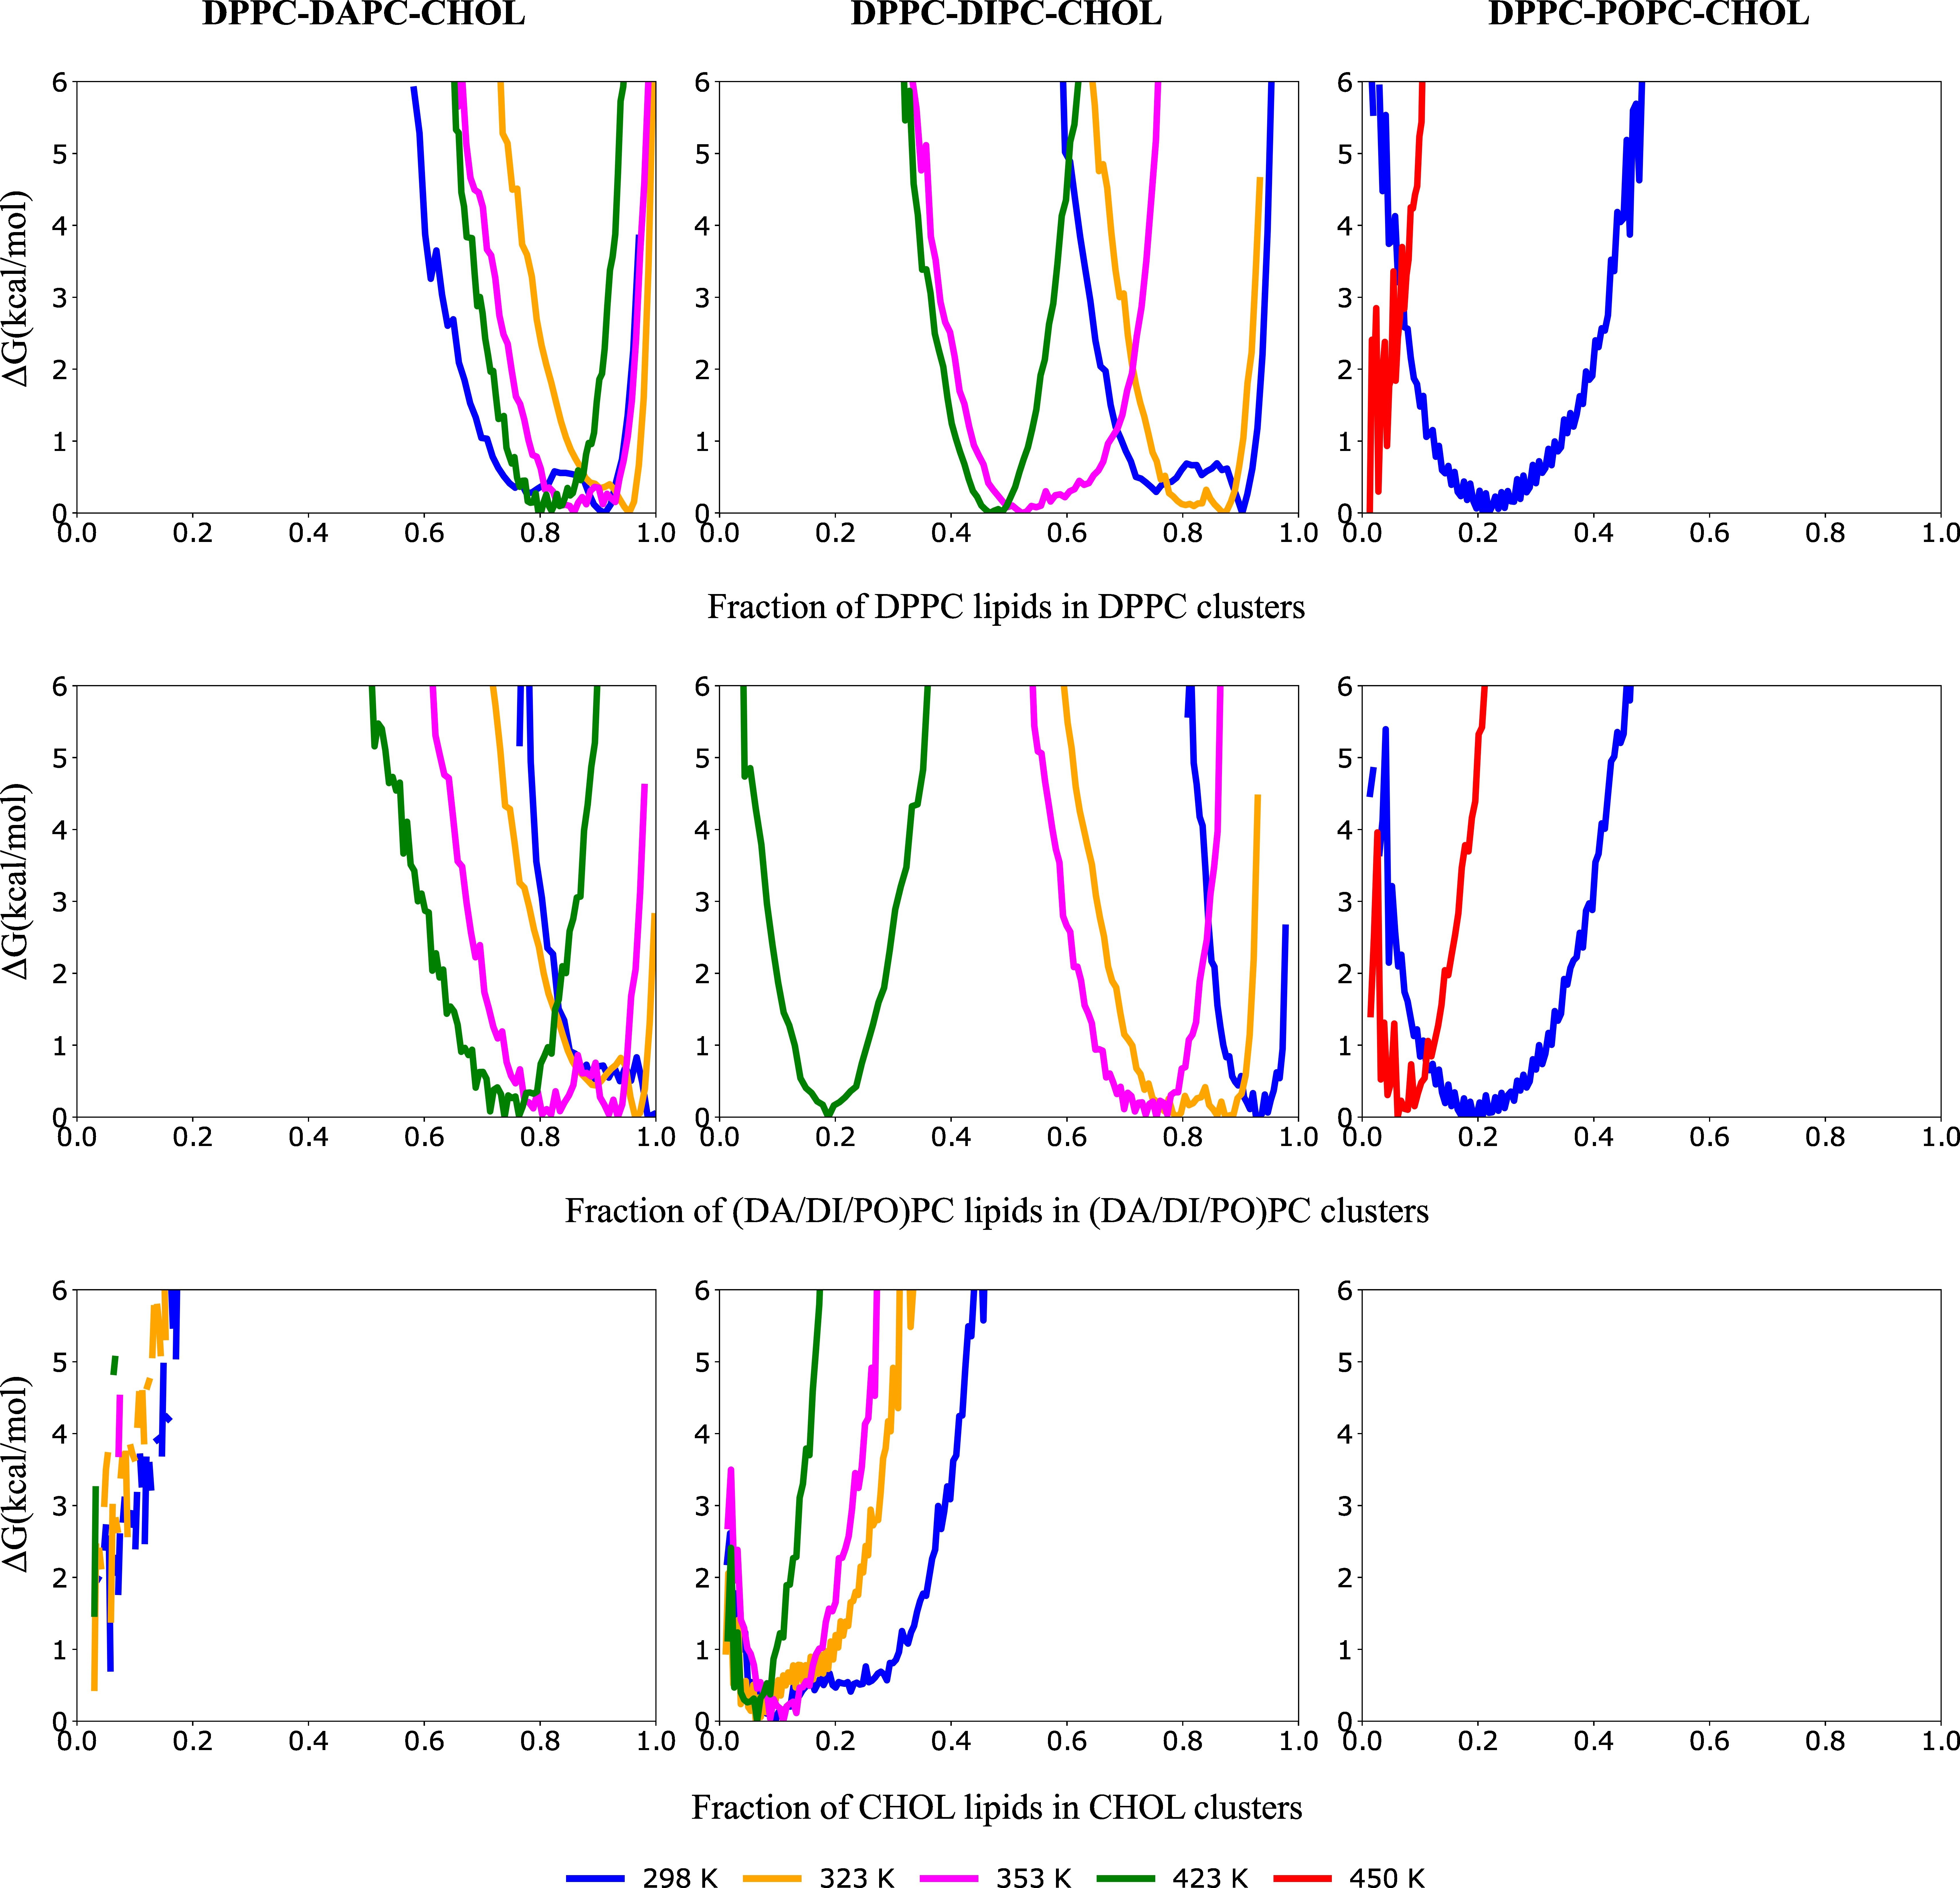
\includegraphics[width=6.5in]{Figures/Supplementary/AVs/SpeciesWiseFLC/placeholder.jpg}
    \caption{Species wise FLC $\Delta$G profile for each system as a function of temperatures. Each column represents each lipid system under study. The rows represent the saturated, unsaturated and cholesterol species within each system respectively}
    \label{figs3:view}
\end{figure}

\begin{figure}[H]
    \centering
    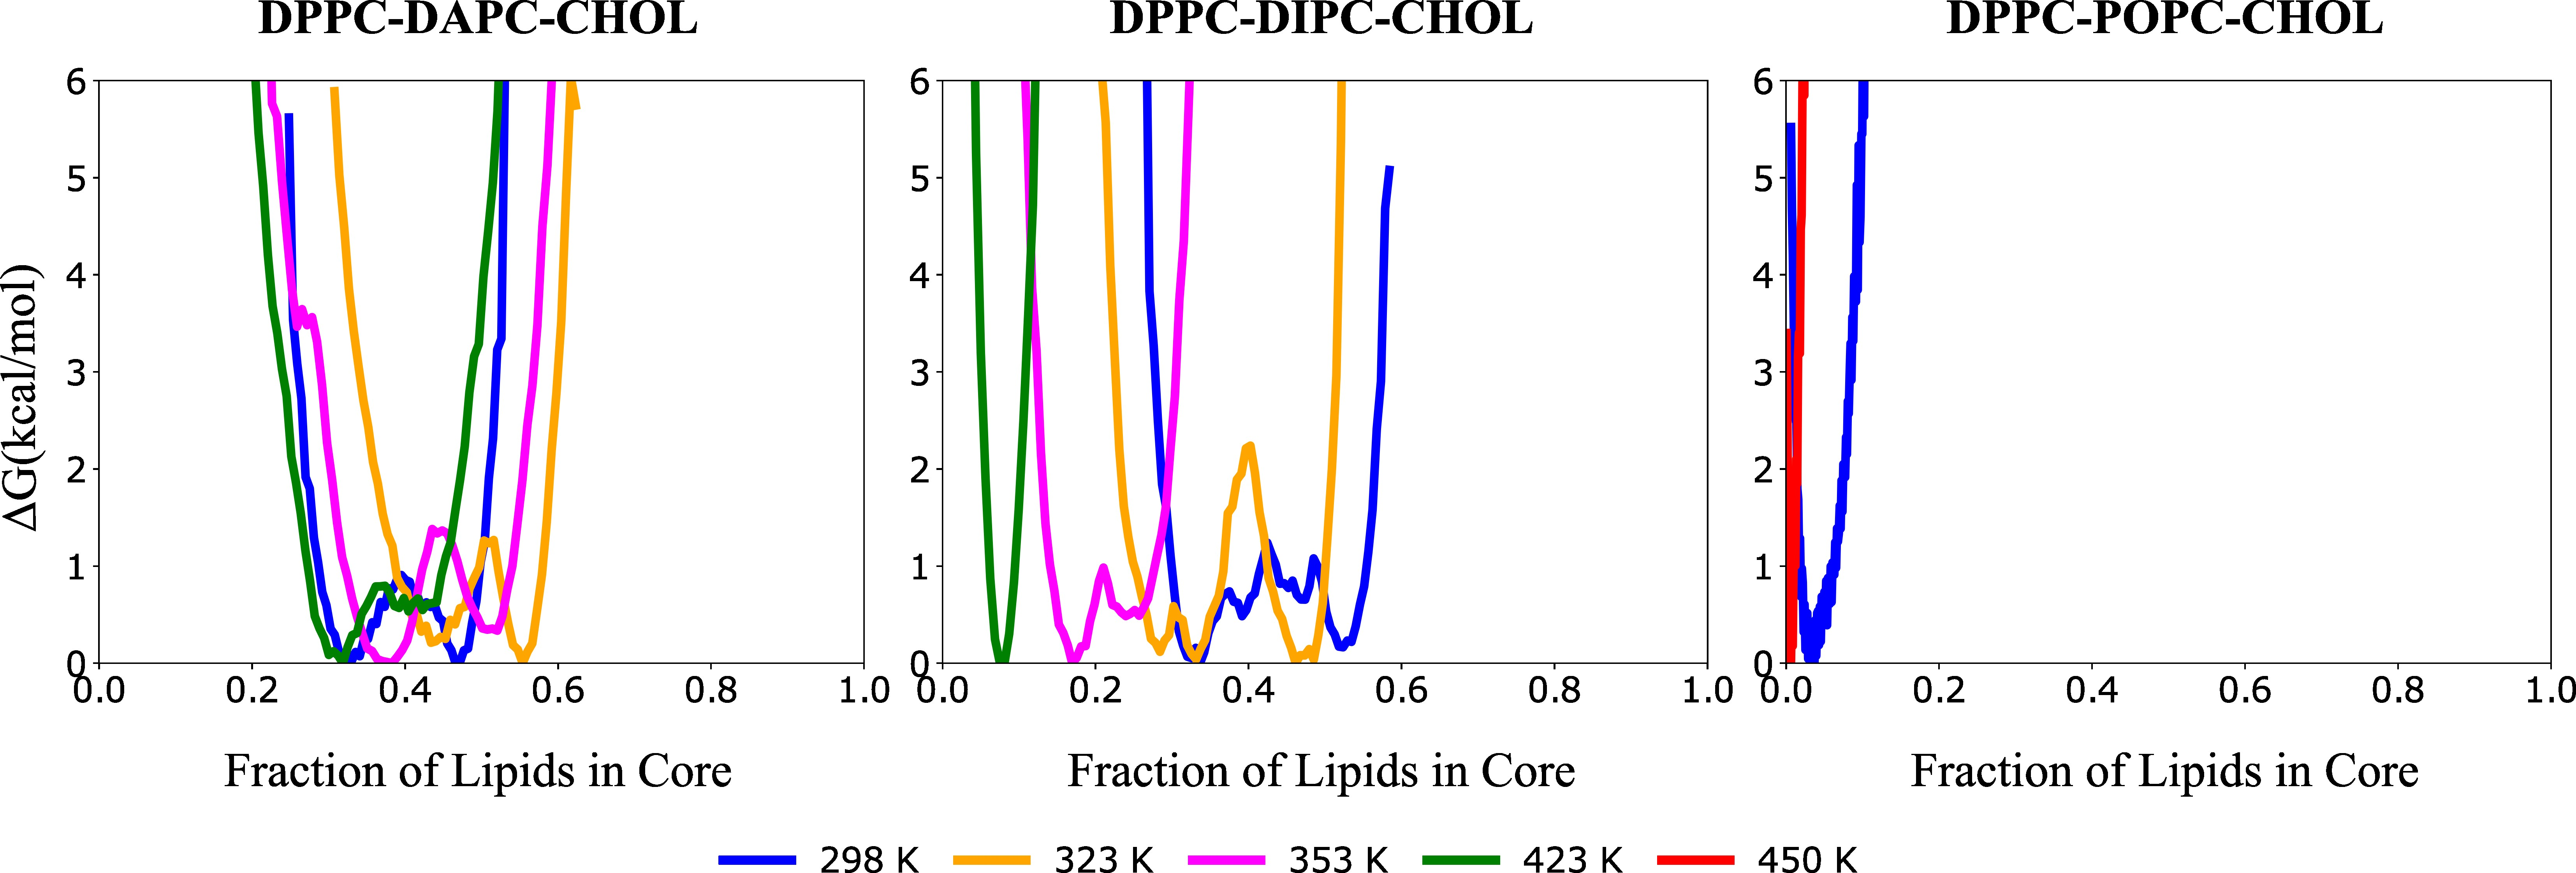
\includegraphics[width=6.5in]{Figures/Supplementary/AVs/FLCore/placeholder.jpg}
    \caption{Fraction of Lipids in Core $\Delta$G profile for each system as a function of temperatures. Each column represents each lipid system under study. The rows represent the total, saturated, unsaturated and cholesterol species within each system respectively}
    \label{figs4:view}
\end{figure}

\begin{figure}[H]
    \centering
    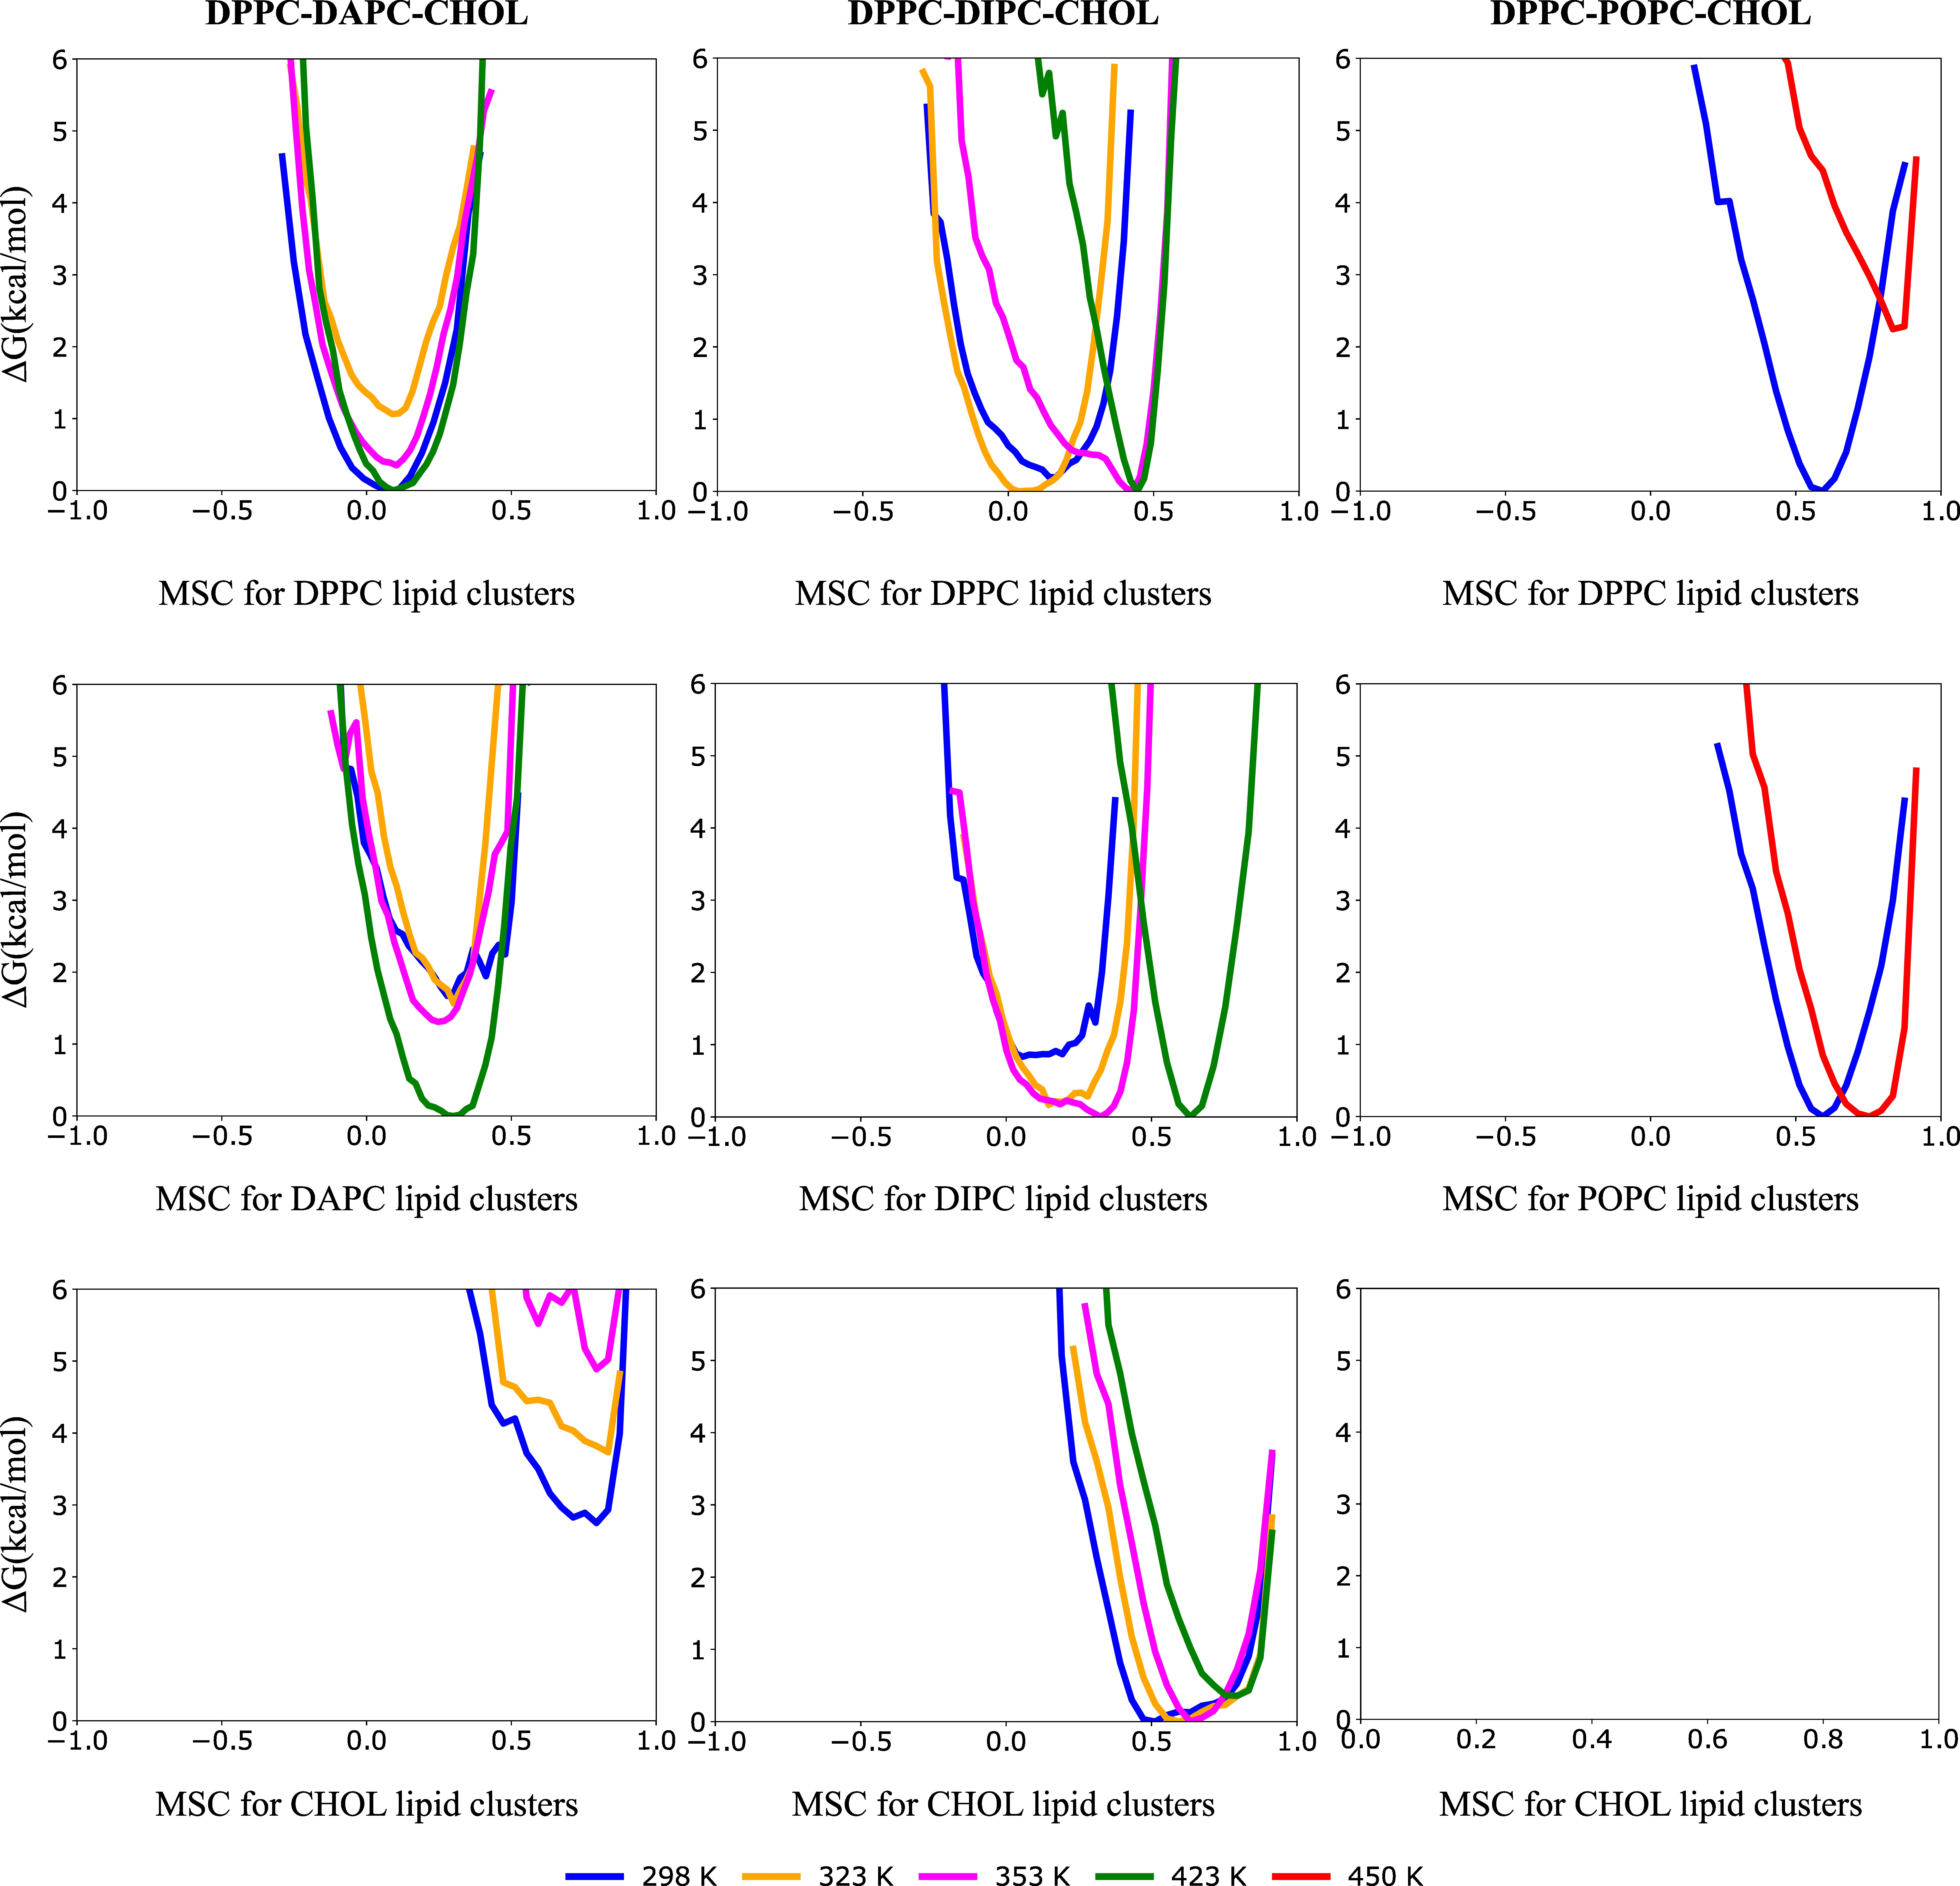
\includegraphics[width=6.5in]{Figures/Supplementary/AVs/MSC/placeholder.jpg}
    \caption{Mean MSC vs. $\Delta$G profile for each system as a function of temperatures. Each column represents each lipid system under study. The rows represent the saturated, unsaturated and cholesterol species within each system respectively}
    \label{figs5:view}
\end{figure}

\section*{Role of cholesterol}

\begin{figure}[H]
    \centering
    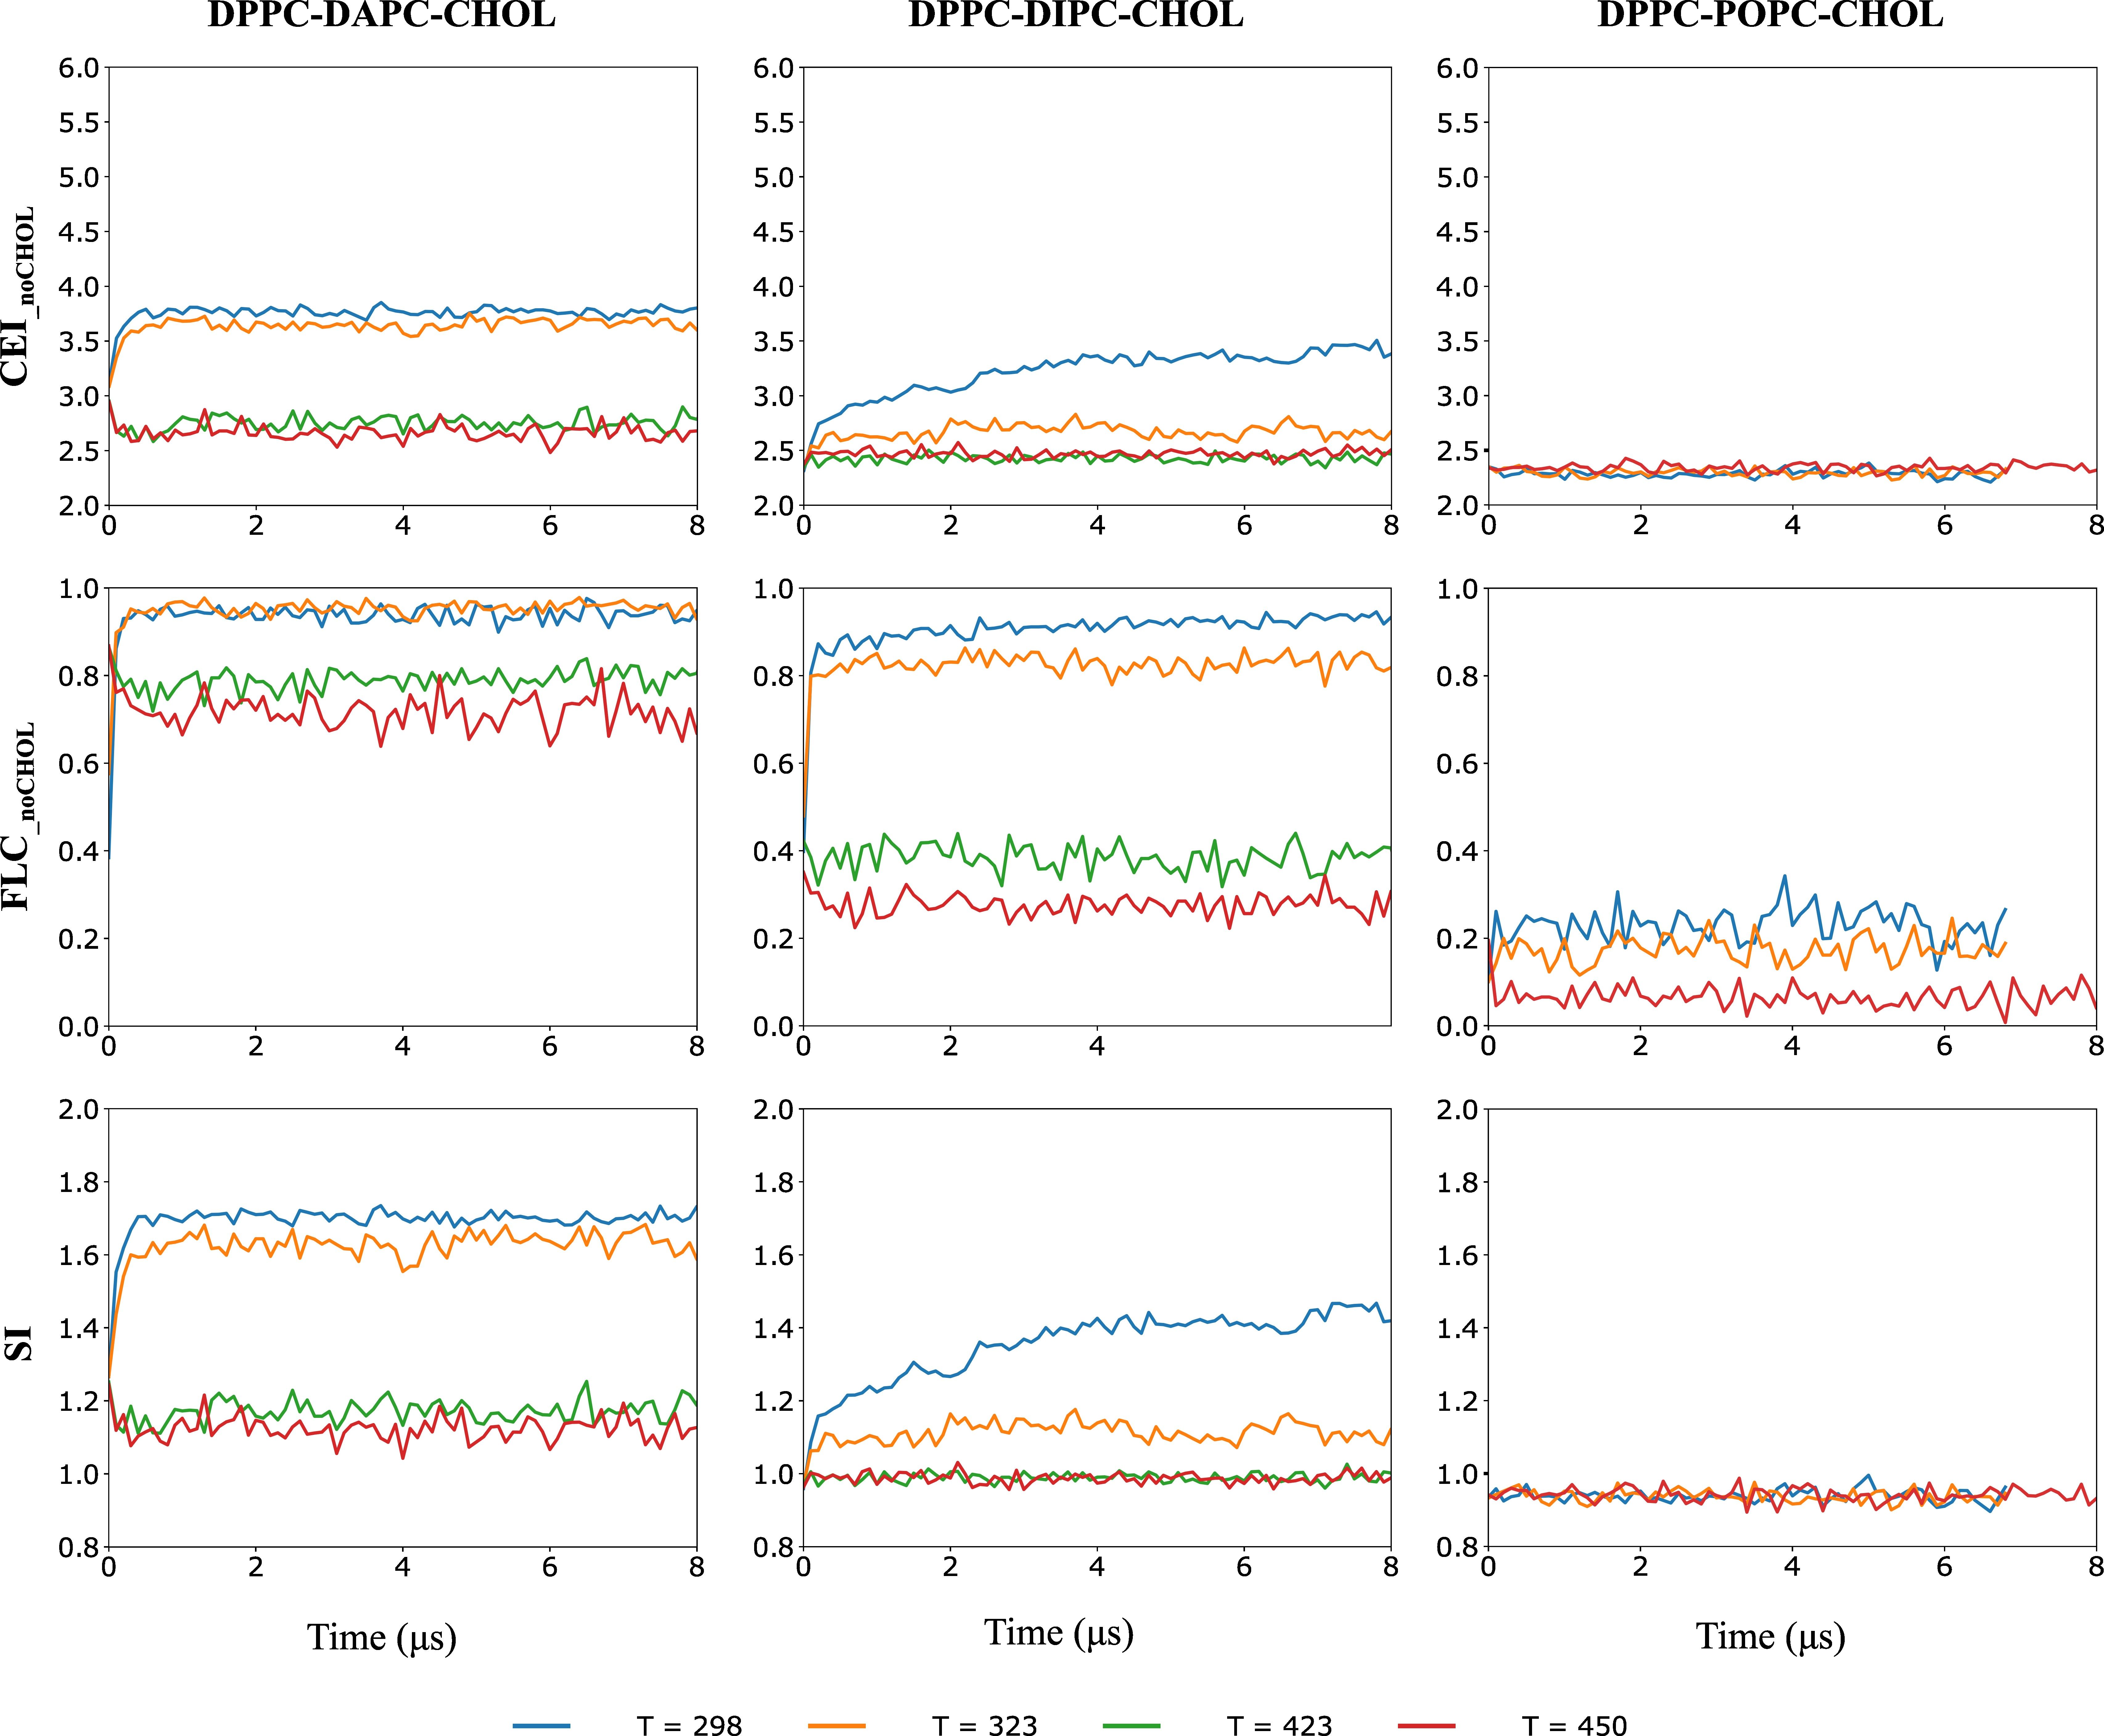
\includegraphics[width=6.5in]{Figures/Supplementary/RoleOfCHOL/placeholder.jpg}
    \caption{Complementary plots to the Fig 3 in Main Article that illustrates the role of cholesterol in CV calculation. Each column represents each lipid system under study. The first two rows represents CEI and FLC without the cholesterol contribution. While the third row represents SI with cholesterol contribution}
    \label{figss6:view}
\end{figure}

\section*{Convergence of free energy curves across replicas}

\begin{figure}[H]
    \centering
    \includegraphics[width=6.5in]{Figures/Supplementary/ReplicaConvergence/placeholder.jpg}
    \caption{The convergence between four replicas of the system at different temperatures. Each column represents each lipid system under study.}
    \label{figs7:view}
\end{figure}

\section*{Interpretating $\Delta\Delta$G estimation}

\begin{figure}[H]
    \centering
    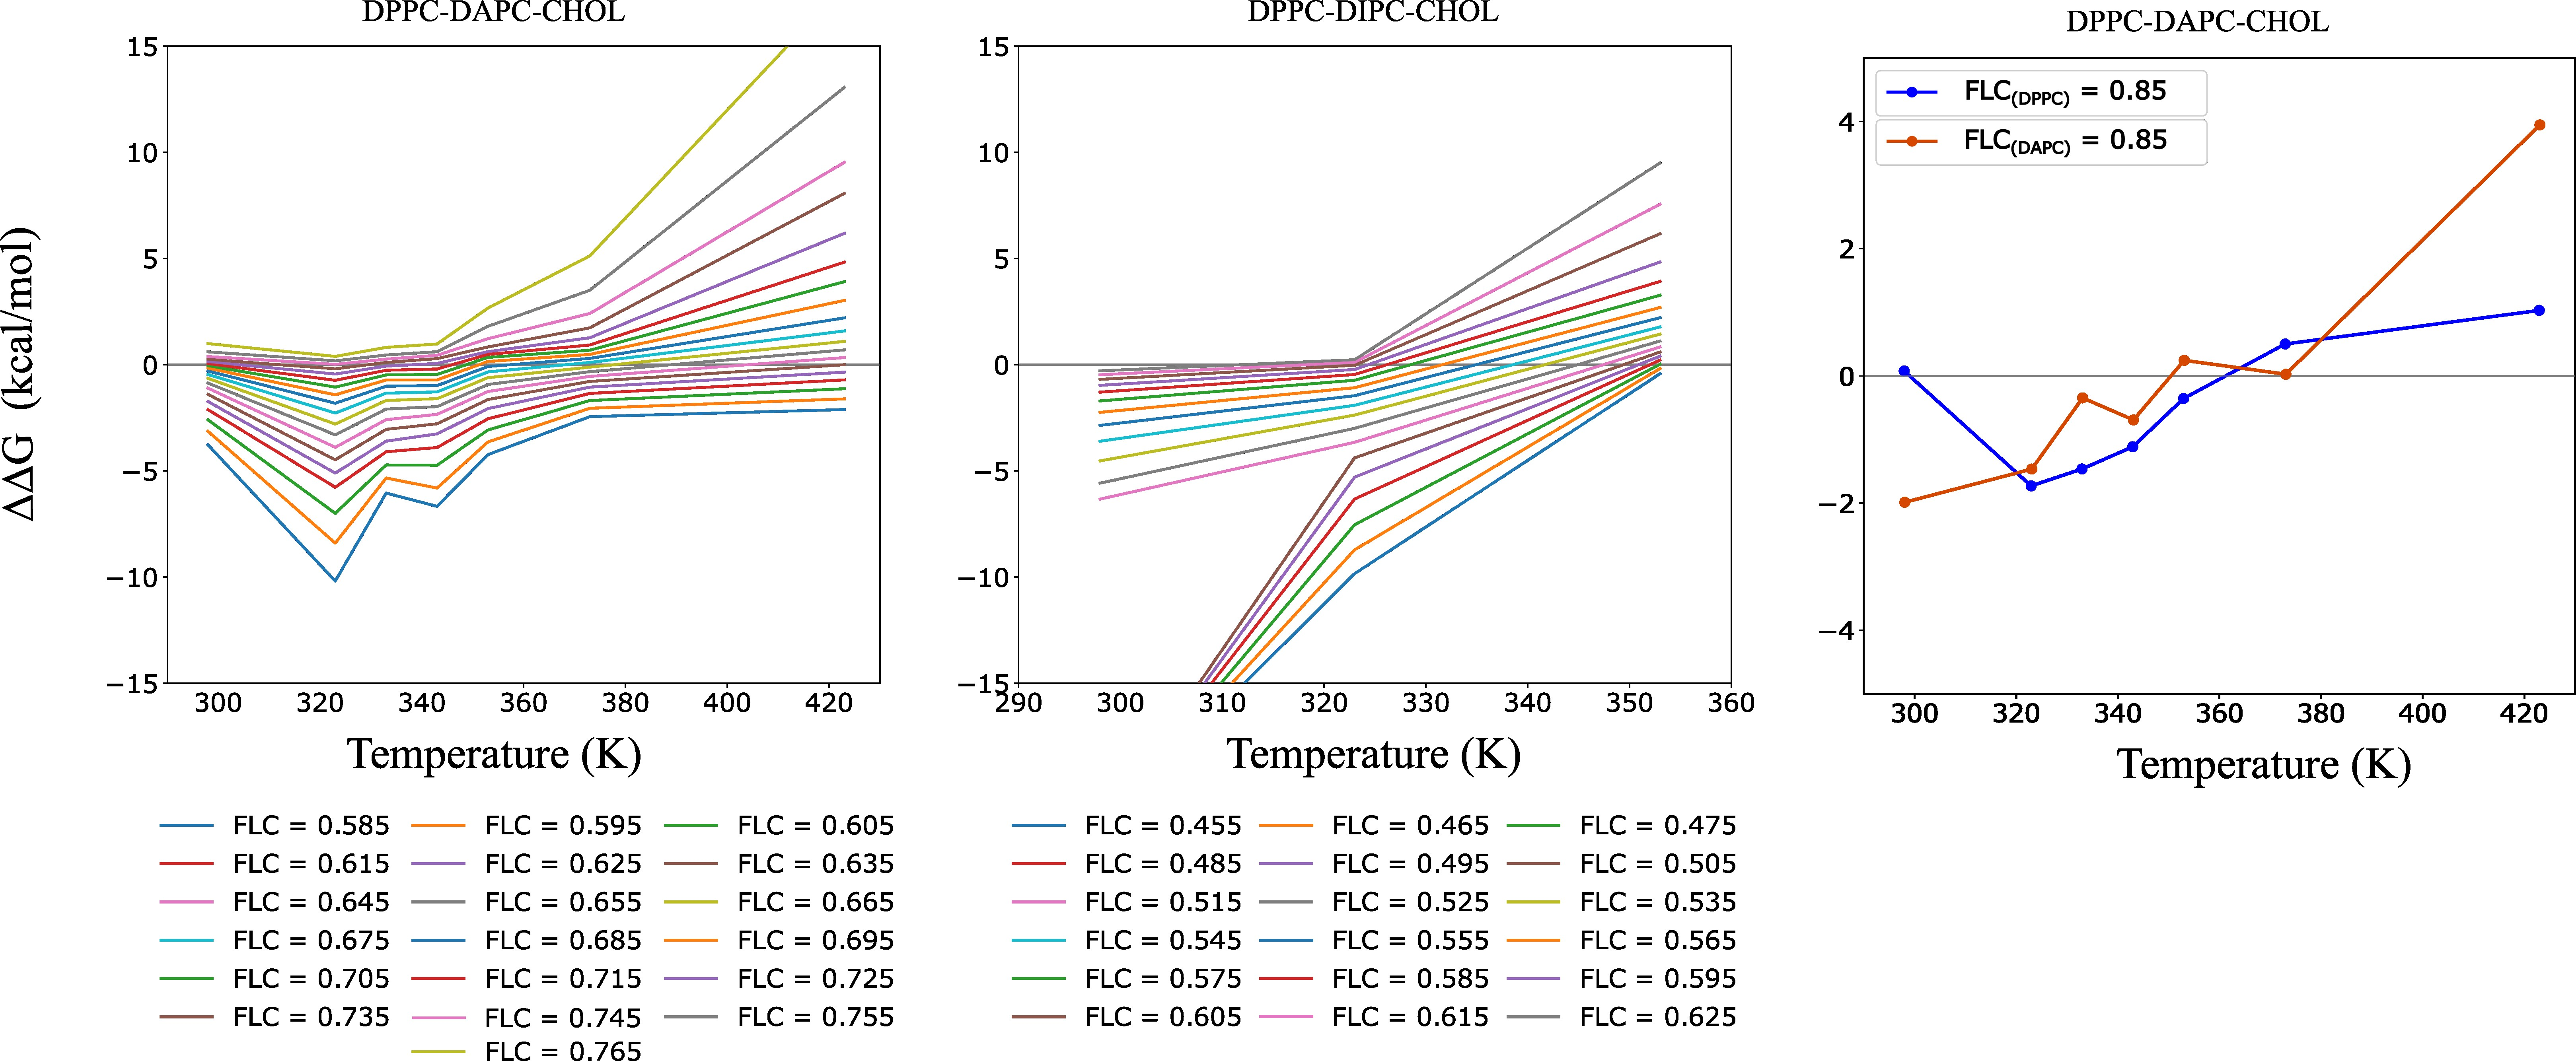
\includegraphics[width=6.5in]{Figures/Supplementary/InterpretingDelDelG/placeholder.jpg}
    \caption{}
    \label{figs8:view}
\end{figure}

\bibliographystyle{unsrt}
\bibliography{PhaseSeparationArticle}


\end{document}